\documentclass[journal,12pt,twocolumn]{IEEEtran}
%
\usepackage{setspace}
\usepackage{gensymb}
\usepackage{xcolor}
\usepackage{caption}
\usepackage[hyphens,spaces,obeyspaces]{url}
%\usepackage{subcaption}
%\doublespacing
\singlespacing

%\usepackage{graphicx}
%\usepackage{amssymb}
%\usepackage{relsize}
\usepackage[cmex10]{amsmath}
\usepackage{mathtools}
%\usepackage{amsthm}
%\interdisplaylinepenalty=2500
%\savesymbol{iint}
%\usepackage{txfonts}
%\restoresymbol{TXF}{iint}
%\usepackage{wasysym}
\usepackage{amsthm}
\usepackage{mathrsfs}
\usepackage{txfonts}
\usepackage{stfloats}
\usepackage{cite}
\usepackage{cases}
\usepackage{subfig}
%\usepackage{xtab}
\usepackage{longtable}
\usepackage{multirow}
%\usepackage{algorithm}
%\usepackage{algpseudocode}
\usepackage{enumerate}
\usepackage{mathtools}
%\usepackage{eenrc}
%\usepackage[framemethod=tikz]{mdframed}
\usepackage[breaklinks]{hyperref}
%\usepackage{breakcites}
\usepackage{listings}
\usepackage[latin1]{inputenc}                                 %%
\usepackage{color}                                            %%
\usepackage{array}                                            %%
\usepackage{longtable}                                        %%
\usepackage{calc}                                             %%
\usepackage{multirow}                                         %%
\usepackage{hhline}                                           %%
\usepackage{ifthen}                                           %%
%optionally (for landscape tables embedded in another document): %%
\usepackage{lscape}     

\usepackage{tikz}
\usepackage{circuitikz}
\usepackage{karnaugh-map}
\usepackage{pgf}
\usepackage[hyphenbreaks]{breakurl}

%\usepackage{url}
%\def\UrlBreaks{\do\/\do-}





%\usepackage{stmaryrd}


%\usepackage{wasysym}
%\newcounter{MYtempeqncnt}
\DeclareMathOperator*{\Res}{Res}
%\renewcommand{\baselinestretch}{2}
\renewcommand\thesection{\arabic{section}}
\renewcommand\thesubsection{\thesection.\arabic{subsection}}
\renewcommand\thesubsubsection{\thesubsection.\arabic{subsubsection}}

\renewcommand\thesectiondis{\arabic{section}}
\renewcommand\thesubsectiondis{\thesectiondis.\arabic{subsection}}
\renewcommand\thesubsubsectiondis{\thesubsectiondis.\arabic{subsubsection}}

% correct bad hyphenation here
\hyphenation{op-tical net-works semi-conduc-tor}

%\lstset{
	%language=C,
	%frame=single, 
	%breaklines=true
	%}

%\lstset{
	%%basicstyle=\small\ttfamily\bfseries,
	%%numberstyle=\small\ttfamily,
	%language=Octave,
	%backgroundcolor=\color{white},
	%%frame=single,
	%%keywordstyle=\bfseries,
	%%breaklines=true,
	%%showstringspaces=false,
	%%xleftmargin=-10mm,
	%%aboveskip=-1mm,
	%%belowskip=0mm
	%}

%\surroundwithmdframed[width=\columnwidth]{lstlisting}
\def\inputGnumericTable{}                                 %%
\lstset{
	%language=C,
	frame=single, 
	breaklines=true,
	columns=fullflexible
}
\graphicspath{ {./title/} } 

\begin{document}
	%
	
	\theoremstyle{definition}
	\newtheorem{theorem}{Theorem}[section]
	\newtheorem{problem}{Problem}
	\newtheorem{proposition}{Proposition}[section]
	\newtheorem{lemma}{Lemma}[section]
	\newtheorem{corollary}[theorem]{Corollary}
	\newtheorem{example}{Example}[section]
	\newtheorem{definition}{Definition}[section]
	%\newtheorem{algorithm}{Algorithm}[section]
	%\newtheorem{cor}{Corollary}
	\newcommand{\BEQA}{\begin{eqnarray}}
		\newcommand{\EEQA}{\end{eqnarray}}
	\newcommand{\define}{\stackrel{\triangle}{=}}
	
	\bibliographystyle{IEEEtran}
	%\bibliographystyle{ieeetr}
	
	\providecommand{\nCr}[2]{\,^{#1}C_{#2}} % nCr
	\providecommand{\nPr}[2]{\,^{#1}P_{#2}} % nPr
	\providecommand{\mbf}{\mathbf}
	\providecommand{\pr}[1]{\ensuremath{\Pr\left(#1\right)}}
	\providecommand{\qfunc}[1]{\ensuremath{Q\left(#1\right)}}
	\providecommand{\sbrak}[1]{\ensuremath{{}\left[#1\right]}}
	\providecommand{\lsbrak}[1]{\ensuremath{{}\left[#1\right.}}
	\providecommand{\rsbrak}[1]{\ensuremath{{}\left.#1\right]}}
	\providecommand{\brak}[1]{\ensuremath{\left(#1\right)}}
	\providecommand{\lbrak}[1]{\ensuremath{\left(#1\right.}}
	\providecommand{\rbrak}[1]{\ensuremath{\left.#1\right)}}
	\providecommand{\cbrak}[1]{\ensuremath{\left\{#1\right\}}}
	\providecommand{\lcbrak}[1]{\ensuremath{\left\{#1\right.}}
	\providecommand{\rcbrak}[1]{\ensuremath{\left.#1\right\}}}
	\providecommand{\ceil}[1]{\left \lceil #1 \right \rceil }
	\theoremstyle{remark}
	\newtheorem{rem}{Remark}
	\newcommand{\sgn}{\mathop{\mathrm{sgn}}}
	\providecommand{\abs}[1]{\left\vert#1\right\vert}
	\providecommand{\res}[1]{\Res\displaylimits_{#1}} 
	\providecommand{\norm}[1]{\lVert#1\rVert}
	\providecommand{\mtx}[1]{\mathbf{#1}}
	\providecommand{\mean}[1]{E\left[ #1 \right]}
	\providecommand{\fourier}{\overset{\mathcal{F}}{ \rightleftharpoons}}
	%\providecommand{\hilbert}{\overset{\mathcal{H}}{ \rightleftharpoons}}
	\providecommand{\system}{\overset{\mathcal{H}}{ \longleftrightarrow}}
	%\newcommand{\solution}[2]{\textbf{Solution:}{#1}}
	\newcommand{\solution}{\noindent \textbf{Solution: }}
	\providecommand{\dec}[2]{\ensuremath{\overset{#1}{\underset{#2}{\gtrless}}}}
	%\numberwithin{equation}{subsection}
	\numberwithin{equation}{section}
	%\numberwithin{problem}{subsection}
	%\numberwithin{definition}{subsection}
	\makeatletter
	\@addtoreset{figure}{problem}
	\makeatother
	
	\let\StandardTheFigure\thefigure
	%\renewcommand{\thefigure}{\theproblem.\arabic{figure}}
	\renewcommand{\thefigure}{\theproblem}
	
	
	%\numberwithin{figure}{subsection}
	
	%\numberwithin{equation}{subsection}
	%\numberwithin{equation}{section}
	%%\numberwithin{equation}{problem}
	%%\numberwithin{problem}{subsection}
	\numberwithin{problem}{section}
	%%\numberwithin{definition}{subsection}
	%\makeatletter
	%\@addtoreset{figure}{problem}
	%\makeatother
	\makeatletter
	\@addtoreset{table}{problem}
	\makeatother
	
	\let\StandardTheFigure\thefigure
	\let\StandardTheTable\thetable
	%%\renewcommand{\thefigure}{\theproblem.\arabic{figure}}
	%\renewcommand{\thefigure}{\theproblem}
	\renewcommand{\thetable}{\theproblem}
	%%\numberwithin{figure}{section}
	
	%%\numberwithin{figure}{subsection}
	
	\vspace{3cm}
	
	\title{
		
		\centering
		
\includegraphics[width=15cm, height=4cm]{title}
		\centering
		
	}
	
	
	
	% paper title
	% can use linebreaks \\ within to get better formatting as desired
	%\title{Matrix Analysis through Octave}
	%
	%
	% author names and IEEE memberships
	% note positions of commas and nonbreaking spaces ( ~ ) LaTeX will not break
	% a structure at a ~ so this keeps an author's name from being broken across
	% two lines.
	% use \thanks{} to gain access to the first footnote area
	% a separate \thanks must be used for each paragraph as LaTeX2e's \thanks
	% was not built to handle multiple paragraphs
	%
	
	\author{G V V Sharma$^{*}$% <-this % stops a space
		\thanks{*The author is with the Department
			of Electrical Engineering, Indian Institute of Technology, Hyderabad
			502285 India e-mail:  gadepall@iith.ac.in. All content in this manual is released under GNU GPL.  Free and open source.}% <-this % stops a space
		%\thanks{J. Doe and J. Doe are with Anonymous University.}% <-this % stops a space
		%\thanks{Manuscript received April 19, 2005; revised January 11, 2007.}}
}
% note the % following the last \IEEEmembership and also \thanks - 
% these prevent an unwanted space from occurring between the last author name
% and the end of the author line. i.e., if you had this:
% 
% \author{....lastname \thanks{...} \thanks{...} }
%                     ^------------^------------^----Do not want these spaces!
%
% a space would be appended to the last name and could cause every name on that
% line to be shifted left slightly. This is one of those "LaTeX things". For
% instance, "\textbf{A} \textbf{B}" will typeset as "A B" not "AB". To get
% "AB" then you have to do: "\textbf{A}\textbf{B}"
% \thanks is no different in this regard, so shield the last } of each \thanks
% that ends a line with a % and do not let a space in before the next \thanks.
% Spaces after \IEEEmembership other than the last one are OK (and needed) as
% you are supposed to have spaces between the names. For what it is worth,
% this is a minor point as most people would not even notice if the said evil
% space somehow managed to creep in.



% The paper headers
%\markboth{Journal of \LaTeX\ Class Files,~Vol.~6, No.~1, January~2007}%
%{Shell \MakeLowercase{\textit{et al.}}: Bare Demo of IEEEtran.cls for Journals}
% The only time the second header will appear is for the odd numbered pages
% after the title page when using the twoside option.
% 
% *** Note that you probably will NOT want to include the author's ***
% *** name in the headers of peer review papers.                   ***
% You can use \ifCLASSOPTIONpeerreview for conditional compilation here if
% you desire.




% If you want to put a publisher's ID mark on the page you can do it like
% this:
%\IEEEpubid{0000--0000/00\$00.00~\copyright~2007 IEEE}
% Remember, if you use this you must call \IEEEpubidadjcol in the second
% column for its text to clear the IEEEpubid mark.



% make the title area
\maketitle

\tableofcontents

\bigskip

\renewcommand{\thefigure}{\theenumi}
\renewcommand{\thetable}{\theenumi}


\begin{abstract}
%\boldmath
This manual explains state machines by deconstructing a decade counter.
\end{abstract}

\section{The Decade Counter}
The block diagram of a decade counter (repeatedly counts up from 0 to 9)
is available in Fig. \ref{fig:dec_counter}.  The {\em incrementing } decoder
and {\em display} decoder are part of {\em combinational} logic, while
the {\em delay} is part of {\em sequential} logic.
\begin{figure}[!h]
	\begin{center}
	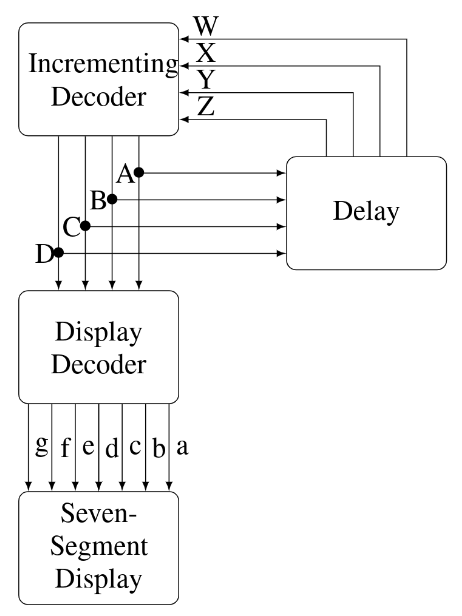
\includegraphics[width=7cm,height=10cm]{./decade}
\end{center}
\caption{The decade counter}
\label{fig:dec_counter}
\end{figure}
%
\section{Finite State Machine}
%
\begin{enumerate}[1.]

\item Fig. \ref{fig:fsm_counter} shows a {\em finite state machine} (FSM) diagram for the decade counter in Fig. \ref{fig:dec_counter}.  $s_0$ is the state when the input to the incrementing decoder is 0.  The {\em state transition table} for the FSM is Table 0 in \cite{gvv_kmap} where the present state is denoted by the variables $W,X,Y,Z$ and the next state by $A,B,C,D$.  
\begin{figure}[!h]
	
	\centering
	\resizebox {\columnwidth} {!} {
		\usetikzlibrary{arrows,automata, positioning, calc}
%\usetikzlibrary{arrows,automata, calc}
%\begin{tikzpicture}[->,shorten >=1pt,node distance=2cm,on grid,auto] 
\begin{tikzpicture}[->,auto] 
   \node[ ] (s_00)   {}; 
   \foreach \i [count=\ni from 1] in {36,72,...,324}
%       \node[state] (s_\ni) [above right = {2*sin(\i)} and {2*(cos(\i)} of s_00]  {\ni};
        \node[state] (s_\ni) [above right = {2*sin(\i)} and {2*(cos(\i)} of s_00]  {$s_{\ni}$};        
        
        \node[state,initial] (s_0) [above right = {0} and {2} of s_00]  {$s_0$};     

   \foreach \i  [count=\j from 1] in {0,1,...,8}
		\path	(s_\i) edge [bend right]  (s_\j) ;

		\path	(s_9) edge [bend right]  (s_0) ;		
           
\end{tikzpicture}

		}
	\caption{FSM for the decade counter.}
	\label{fig:fsm_counter}
\end{figure}
\item The FSM implementation is available in Fig. \ref{fig:dff}.  The {\em flip-flops} hold the input for the time that is given by the {\em clock}.  This is nothing but the implementation of the {\em Delay} block in Fig. \ref{fig:dec_counter}.
%
\begin{figure}[!h]
	\begin{center}
	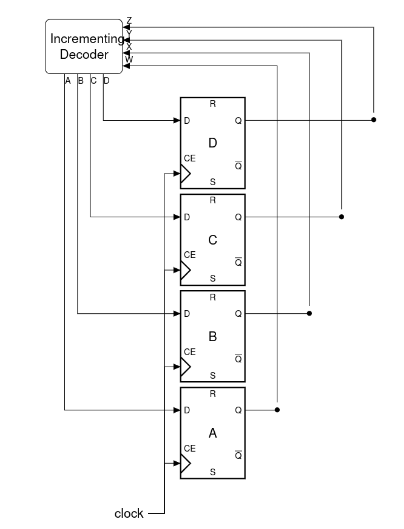
\includegraphics[width=7cm,height=9cm]{./fsm}
\end{center}
	\caption{Decade counter FSM implementation using D-Flip Flops.}
	\label{fig:dff}
\end{figure}
%
\item The hardware cost of the system is given by
\begin{equation}
	\text{No. of D Flip-Flops} = \ceil{\log_{2}\brak{\text{No. of States}}}
\end{equation}
For the FSM in Fig. \ref{fig:fsm_counter}, the number of states is 9, hence the number flipflops required = 4.  
\item Draw the state transition diagram for 
a decade down counter (counts from 9 to 0 repeatedly) using an FSM.  \\
\textbf{Solution:} Refer \ref{fig:fsm_down}\\
\begin{figure}
	

\begin{center}
	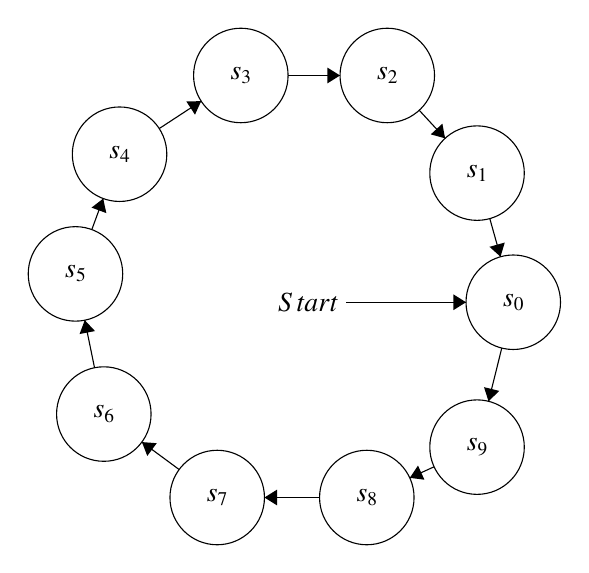
\begin{tikzpicture}[scale=0.2]
		\tikzstyle{every node}+=[inner sep=0pt]
		\draw [black] (43.8,-12.7) circle (3);
		\draw (43.8,-12.7) node {$s_2$};
		\draw [black] (49.5,-18.9) circle (3);
		\draw (49.5,-18.9) node {$s_1$};
		\draw [black] (24,-25.3) circle (3);
		\draw (24,-25.3) node {$s_5$};
		\draw [black] (51.8,-27.1) circle (3);
		\draw (51.8,-27.1) node {$s_0$};
		\draw [black] (34.5,-12.7) circle (3);
		\draw (34.5,-12.7) node {$s_3$};
		\draw [black] (26.8,-17.7) circle (3);
		\draw (26.8,-17.7) node {$s_4$};
		\draw [black] (25.8,-34.2) circle (3);
		\draw (25.8,-34.2) node {$s_6$};
		\draw [black] (33,-39.5) circle (3);
		\draw (33,-39.5) node {$s_7$};
		\draw [black] (42.5,-39.5) circle (3);
		\draw (42.5,-39.5) node {$s_8$};
		\draw [black] (49.5,-36.3) circle (3);
		\draw (49.5,-36.3) node {$s_9$};
		\draw [black] (25.04,-22.48) -- (25.76,-20.52);
		\fill [black] (25.76,-20.52) -- (25.02,-21.09) -- (25.96,-21.44);
		\draw [black] (51.07,-30.01) -- (50.23,-33.39);
		\fill [black] (50.23,-33.39) -- (50.91,-32.73) -- (49.94,-32.49);
		\draw [black] (46.77,-37.55) -- (45.23,-38.25);
		\fill [black] (45.23,-38.25) -- (46.16,-38.37) -- (45.75,-37.47);
		\draw [black] (39.5,-39.5) -- (36,-39.5);
		\fill [black] (36,-39.5) -- (36.8,-40) -- (36.8,-39);
		\draw [black] (30.58,-37.72) -- (28.22,-35.98);
		\fill [black] (28.22,-35.98) -- (28.56,-36.86) -- (29.16,-36.05);
		\draw [black] (25.21,-31.26) -- (24.59,-28.24);
		\fill [black] (24.59,-28.24) -- (24.26,-29.12) -- (25.24,-28.93);
		\draw [black] (29.32,-16.07) -- (31.98,-14.33);
		\fill [black] (31.98,-14.33) -- (31.04,-14.35) -- (31.59,-15.19);
		\draw [black] (45.83,-14.91) -- (47.47,-16.69);
		\fill [black] (47.47,-16.69) -- (47.3,-15.76) -- (46.56,-16.44);
		\draw [black] (50.31,-21.79) -- (50.99,-24.21);
		\fill [black] (50.99,-24.21) -- (51.26,-23.31) -- (50.29,-23.58);
		\draw [black] (37.5,-12.7) -- (40.8,-12.7);
		\fill [black] (40.8,-12.7) -- (40,-12.2) -- (40,-13.2);
		\draw [black] (41.2,-27.1) -- (48.8,-27.1);
		\draw (40.7,-27.1) node [left] {$Start$};
		\fill [black] (48.8,-27.1) -- (48,-26.6) -- (48,-27.6);
	\end{tikzpicture}
\caption{FSM for Down Counter}
\label{fig:fsm_down}
\end{center}
\end{figure}
\item Write the state transition table for the down counter.\\
\textbf{Solution:}\\
Without Don't Care: Refer \ref{table:counter_decoder}\\
With Don't Care: Refer \ref{table:dont_care_table}
\begin{table}[!h]
	\centering	
	%%%%%%%%%%%%%%%%%%%%%%%%%%%%%%%%%%%%%%%%%%%%%%%%%%%%%%%%%%%%%%%%%%%%%%
%%                                                                  %%
%%  This is the header of a LaTeX2e file exported from Gnumeric.    %%
%%                                                                  %%
%%  This file can be compiled as it stands or included in another   %%
%%  LaTeX document. The table is based on the longtable package so  %%
%%  the longtable options (headers, footers...) can be set in the   %%
%%  preamble section below (see PRAMBLE).                           %%
%%                                                                  %%
%%  To include the file in another, the following two lines must be %%
%%  in the including file:                                          %%
%%        \def\inputGnumericTable{}                                 %%
%%  at the beginning of the file and:                               %%
%%        \input{name-of-this-file.tex}                             %%
%%  where the table is to be placed. Note also that the including   %%
%%  file must use the following packages for the table to be        %%
%%  rendered correctly:                                             %%
%%    \usepackage[latin1]{inputenc}                                 %%
%%    \usepackage{color}                                            %%
%%    \usepackage{array}                                            %%
%%    \usepackage{longtable}                                        %%
%%    \usepackage{calc}                                             %%
%%    \usepackage{multirow}                                         %%
%%    \usepackage{hhline}                                           %%
%%    \usepackage{ifthen}                                           %%
%%  optionally (for landscape tables embedded in another document): %%
%%    \usepackage{lscape}                                           %%
%%                                                                  %%
%%%%%%%%%%%%%%%%%%%%%%%%%%%%%%%%%%%%%%%%%%%%%%%%%%%%%%%%%%%%%%%%%%%%%%



%%  This section checks if we are begin input into another file or  %%
%%  the file will be compiled alone. First use a macro taken from   %%
%%  the TeXbook ex 7.7 (suggestion of Han-Wen Nienhuys).            %%
\def\ifundefined#1{\expandafter\ifx\csname#1\endcsname\relax}


%%  Check for the \def token for inputed files. If it is not        %%
%%  defined, the file will be processed as a standalone and the     %%
%%  preamble will be used.                                          %%
\ifundefined{inputGnumericTable}

%%  We must be able to close or not the document at the end.        %%
	\def\gnumericTableEnd{\end{document}}


%%%%%%%%%%%%%%%%%%%%%%%%%%%%%%%%%%%%%%%%%%%%%%%%%%%%%%%%%%%%%%%%%%%%%%
%%                                                                  %%
%%  This is the PREAMBLE. Change these values to get the right      %%
%%  paper size and other niceties.                                  %%
%%                                                                  %%
%%%%%%%%%%%%%%%%%%%%%%%%%%%%%%%%%%%%%%%%%%%%%%%%%%%%%%%%%%%%%%%%%%%%%%

	\documentclass[12pt%
			  %,landscape%
                    ]{report}
       \usepackage[latin1]{inputenc}
       \usepackage{fullpage}
       \usepackage{color}
       \usepackage{array}
       \usepackage{longtable}
       \usepackage{calc}
       \usepackage{multirow}
       \usepackage{hhline}
       \usepackage{ifthen}

	\begin{document}


%%  End of the preamble for the standalone. The next section is for %%
%%  documents which are included into other LaTeX2e files.          %%
\else

%%  We are not a stand alone document. For a regular table, we will %%
%%  have no preamble and only define the closing to mean nothing.   %%
    \def\gnumericTableEnd{}

%%  If we want landscape mode in an embedded document, comment out  %%
%%  the line above and uncomment the two below. The table will      %%
%%  begin on a new page and run in landscape mode.                  %%
%       \def\gnumericTableEnd{\end{landscape}}
%       \begin{landscape}


%%  End of the else clause for this file being \input.              %%
\fi

%%%%%%%%%%%%%%%%%%%%%%%%%%%%%%%%%%%%%%%%%%%%%%%%%%%%%%%%%%%%%%%%%%%%%%
%%                                                                  %%
%%  The rest is the gnumeric table, except for the closing          %%
%%  statement. Changes below will alter the table's appearance.     %%
%%                                                                  %%
%%%%%%%%%%%%%%%%%%%%%%%%%%%%%%%%%%%%%%%%%%%%%%%%%%%%%%%%%%%%%%%%%%%%%%

\providecommand{\gnumericmathit}[1]{#1} 
%%  Uncomment the next line if you would like your numbers to be in %%
%%  italics if they are italizised in the gnumeric table.           %%
%\renewcommand{\gnumericmathit}[1]{\mathit{#1}}
\providecommand{\gnumericPB}[1]%
{\let\gnumericTemp=\\#1\let\\=\gnumericTemp\hspace{0pt}}
 \ifundefined{gnumericTableWidthDefined}
        \newlength{\gnumericTableWidth}
        \newlength{\gnumericTableWidthComplete}
        \newlength{\gnumericMultiRowLength}
        \global\def\gnumericTableWidthDefined{}
 \fi
%% The following setting protects this code from babel shorthands.  %%
 \ifthenelse{\isundefined{\languageshorthands}}{}{\languageshorthands{english}}
%%  The default table format retains the relative column widths of  %%
%%  gnumeric. They can easily be changed to c, r or l. In that case %%
%%  you may want to comment out the next line and uncomment the one %%
%%  thereafter                                                      %%
\providecommand\gnumbox{\makebox[0pt]}
%%\providecommand\gnumbox[1][]{\makebox}

%% to adjust positions in multirow situations                       %%
\setlength{\bigstrutjot}{\jot}
\setlength{\extrarowheight}{\doublerulesep}

%%  The \setlongtables command keeps column widths the same across  %%
%%  pages. Simply comment out next line for varying column widths.  %%
\setlongtables

\setlength\gnumericTableWidth{%
	13pt+%
	12pt+%
	12pt+%
	12pt+%
	12pt+%
	12pt+%
	12pt+%
	12pt+%
0pt}
\def\gumericNumCols{8}
\setlength\gnumericTableWidthComplete{\gnumericTableWidth+%
         \tabcolsep*\gumericNumCols*2+\arrayrulewidth*\gumericNumCols}
\ifthenelse{\lengthtest{\gnumericTableWidthComplete > \linewidth}}%
         {\def\gnumericScale{\ratio{\linewidth-%
                        \tabcolsep*\gumericNumCols*2-%
                        \arrayrulewidth*\gumericNumCols}%
{\gnumericTableWidth}}}%
{\def\gnumericScale{1}}

%%%%%%%%%%%%%%%%%%%%%%%%%%%%%%%%%%%%%%%%%%%%%%%%%%%%%%%%%%%%%%%%%%%%%%
%%                                                                  %%
%% The following are the widths of the various columns. We are      %%
%% defining them here because then they are easier to change.       %%
%% Depending on the cell formats we may use them more than once.    %%
%%                                                                  %%
%%%%%%%%%%%%%%%%%%%%%%%%%%%%%%%%%%%%%%%%%%%%%%%%%%%%%%%%%%%%%%%%%%%%%%

\ifthenelse{\isundefined{\gnumericColA}}{\newlength{\gnumericColA}}{}\settowidth{\gnumericColA}{\begin{tabular}{@{}p{13pt*\gnumericScale}@{}}x\end{tabular}}
\ifthenelse{\isundefined{\gnumericColB}}{\newlength{\gnumericColB}}{}\settowidth{\gnumericColB}{\begin{tabular}{@{}p{13pt*\gnumericScale}@{}}x\end{tabular}}
\ifthenelse{\isundefined{\gnumericColC}}{\newlength{\gnumericColC}}{}\settowidth{\gnumericColC}{\begin{tabular}{@{}p{13pt*\gnumericScale}@{}}x\end{tabular}}
\ifthenelse{\isundefined{\gnumericColD}}{\newlength{\gnumericColD}}{}\settowidth{\gnumericColD}{\begin{tabular}{@{}p{13pt*\gnumericScale}@{}}x\end{tabular}}
\ifthenelse{\isundefined{\gnumericColE}}{\newlength{\gnumericColE}}{}\settowidth{\gnumericColE}{\begin{tabular}{@{}p{13pt*\gnumericScale}@{}}x\end{tabular}}
\ifthenelse{\isundefined{\gnumericColF}}{\newlength{\gnumericColF}}{}\settowidth{\gnumericColF}{\begin{tabular}{@{}p{13pt*\gnumericScale}@{}}x\end{tabular}}
\ifthenelse{\isundefined{\gnumericColG}}{\newlength{\gnumericColG}}{}\settowidth{\gnumericColG}{\begin{tabular}{@{}p{13pt*\gnumericScale}@{}}x\end{tabular}}
\ifthenelse{\isundefined{\gnumericColH}}{\newlength{\gnumericColH}}{}\settowidth{\gnumericColH}{\begin{tabular}{@{}p{13pt*\gnumericScale}@{}}x\end{tabular}}


\begin{tabular}[c]{
%\begin{longtable}[c]{%
	b{\gnumericColA}%
	b{\gnumericColB}%
	b{\gnumericColC}%
	b{\gnumericColD}%
	b{\gnumericColE}%
	b{\gnumericColF}%
	b{\gnumericColG}%
	b{\gnumericColH}%
	}

%%%%%%%%%%%%%%%%%%%%%%%%%%%%%%%%%%%%%%%%%%%%%%%%%%%%%%%%%%%%%%%%%%%%%%
%%  The longtable options. (Caption, headers... see Goosens, p.124) %%
%	\caption{The Table Caption.}             \\	%
% \hline	% Across the top of the table.
%%  The rest of these options are table rows which are placed on    %%
%%  the first, last or every page. Use \multicolumn if you want.    %%

%%  Header for the first page.                                      %%
%	\multicolumn{8}{c}{The First Header} \\ \hline 
%	\multicolumn{1}{c}{colTag}	%Column 1
%	&\multicolumn{1}{c}{colTag}	%Column 2
%	&\multicolumn{1}{c}{colTag}	%Column 3
%	&\multicolumn{1}{c}{colTag}	%Column 4
%	&\multicolumn{1}{c}{colTag}	%Column 5
%	&\multicolumn{1}{c}{colTag}	%Column 6
%	&\multicolumn{1}{c}{colTag}	%Column 7
%	&\multicolumn{1}{c}{colTag}	\\ \hline %Last column
%	\endfirsthead

%%  The running header definition.                                  %%
%	\hline
%	\multicolumn{8}{l}{\ldots\small\slshape continued} \\ \hline
%	\multicolumn{1}{c}{colTag}	%Column 1
%	&\multicolumn{1}{c}{colTag}	%Column 2
%	&\multicolumn{1}{c}{colTag}	%Column 3
%	&\multicolumn{1}{c}{colTag}	%Column 4
%	&\multicolumn{1}{c}{colTag}	%Column 5
%	&\multicolumn{1}{c}{colTag}	%Column 6
%	&\multicolumn{1}{c}{colTag}	%Column 7
%	&\multicolumn{1}{c}{colTag}	\\ \hline %Last column
%	\endhead

%%  The running footer definition.                                  %%
%	\hline
%	\multicolumn{8}{r}{\small\slshape continued\ldots} \\
%	\endfoot

%%  The ending footer definition.                                   %%
%	\multicolumn{8}{c}{That's all folks} \\ \hline 
%	\endlastfoot
%%%%%%%%%%%%%%%%%%%%%%%%%%%%%%%%%%%%%%%%%%%%%%%%%%%%%%%%%%%%%%%%%%%%%%

\hhline{|-|-|-|-|-|-|-|-}
	 \multicolumn{1}{|p{\gnumericColA}|}%
	{\gnumericPB{\centering}\gnumbox{Z}}
	&\multicolumn{1}{p{\gnumericColB}|}%
	{\gnumericPB{\centering}\gnumbox{Y}}
	&\multicolumn{1}{p{\gnumericColC}|}%
	{\gnumericPB{\centering}\gnumbox{X}}
	&\multicolumn{1}{p{\gnumericColD}|}%
	{\gnumericPB{\centering}\gnumbox{W}}
	&\multicolumn{1}{p{\gnumericColE}|}%
	{\gnumericPB{\centering}\gnumbox{\textbf{D}}}
	&\multicolumn{1}{p{\gnumericColF}|}%
	{\gnumericPB{\centering}\gnumbox{\textbf{C}}}
	&\multicolumn{1}{p{\gnumericColG}|}%
	{\gnumericPB{\centering}\gnumbox{\textbf{B}}}
	&\multicolumn{1}{p{\gnumericColH}|}%
	{\gnumericPB{\centering}\gnumbox{\textbf{A}}}
\\
\hhline{|--------|}
	 \multicolumn{1}{|p{\gnumericColA}|}%
	{\gnumericPB{\centering}\gnumbox{0}}
	&\multicolumn{1}{p{\gnumericColB}|}%
	{\gnumericPB{\centering}\gnumbox{0}}
	&\multicolumn{1}{p{\gnumericColC}|}%
	{\gnumericPB{\centering}\gnumbox{0}}
	&\multicolumn{1}{p{\gnumericColD}|}%
	{\gnumericPB{\centering}\gnumbox{0}}
	&\multicolumn{1}{p{\gnumericColE}|}%
	{\gnumericPB{\centering}\gnumbox{\textbf{1}}}
	&\multicolumn{1}{p{\gnumericColF}|}%
	{\gnumericPB{\centering}\gnumbox{\textbf{0}}}
	&\multicolumn{1}{p{\gnumericColG}|}%
	{\gnumericPB{\centering}\gnumbox{\textbf{0}}}
	&\multicolumn{1}{p{\gnumericColH}|}%
	{\gnumericPB{\centering}\gnumbox{\textbf{1}}}
\\
\hhline{|--------|}
	 \multicolumn{1}{|p{\gnumericColA}|}%
	{\gnumericPB{\centering}\gnumbox{1}}
	&\multicolumn{1}{p{\gnumericColB}|}%
	{\gnumericPB{\centering}\gnumbox{0}}
	&\multicolumn{1}{p{\gnumericColC}|}%
	{\gnumericPB{\centering}\gnumbox{0}}
	&\multicolumn{1}{p{\gnumericColD}|}%
	{\gnumericPB{\centering}\gnumbox{1}}
	&\multicolumn{1}{p{\gnumericColE}|}%
	{\gnumericPB{\centering}\gnumbox{\textbf{1}}}
	&\multicolumn{1}{p{\gnumericColF}|}%
	{\gnumericPB{\centering}\gnumbox{\textbf{0}}}
	&\multicolumn{1}{p{\gnumericColG}|}%
	{\gnumericPB{\centering}\gnumbox{\textbf{0}}}
	&\multicolumn{1}{p{\gnumericColH}|}%
	{\gnumericPB{\centering}\gnumbox{\textbf{0}}}
\\
\hhline{|--------|}
	 \multicolumn{1}{|p{\gnumericColA}|}%
	{\gnumericPB{\centering}\gnumbox{1}}
	&\multicolumn{1}{p{\gnumericColB}|}%
	{\gnumericPB{\centering}\gnumbox{0}}
	&\multicolumn{1}{p{\gnumericColC}|}%
	{\gnumericPB{\centering}\gnumbox{0}}
	&\multicolumn{1}{p{\gnumericColD}|}%
	{\gnumericPB{\centering}\gnumbox{0}}
	&\multicolumn{1}{p{\gnumericColE}|}%
	{\gnumericPB{\centering}\gnumbox{\textbf{0}}}
	&\multicolumn{1}{p{\gnumericColF}|}%
	{\gnumericPB{\centering}\gnumbox{\textbf{1}}}
	&\multicolumn{1}{p{\gnumericColG}|}%
	{\gnumericPB{\centering}\gnumbox{\textbf{1}}}
	&\multicolumn{1}{p{\gnumericColH}|}%
	{\gnumericPB{\centering}\gnumbox{\textbf{1}}}
\\
\hhline{|--------|}
	 \multicolumn{1}{|p{\gnumericColA}|}%
	{\gnumericPB{\centering}\gnumbox{0}}
	&\multicolumn{1}{p{\gnumericColB}|}%
	{\gnumericPB{\centering}\gnumbox{1}}
	&\multicolumn{1}{p{\gnumericColC}|}%
	{\gnumericPB{\centering}\gnumbox{1}}
	&\multicolumn{1}{p{\gnumericColD}|}%
	{\gnumericPB{\centering}\gnumbox{1}}
	&\multicolumn{1}{p{\gnumericColE}|}%
	{\gnumericPB{\centering}\gnumbox{\textbf{0}}}
	&\multicolumn{1}{p{\gnumericColF}|}%
	{\gnumericPB{\centering}\gnumbox{\textbf{1}}}
	&\multicolumn{1}{p{\gnumericColG}|}%
	{\gnumericPB{\centering}\gnumbox{\textbf{1}}}
	&\multicolumn{1}{p{\gnumericColH}|}%
	{\gnumericPB{\centering}\gnumbox{\textbf{0}}}
\\
\hhline{|--------|}
	 \multicolumn{1}{|p{\gnumericColA}|}%
	{\gnumericPB{\centering}\gnumbox{0}}
	&\multicolumn{1}{p{\gnumericColB}|}%
	{\gnumericPB{\centering}\gnumbox{1}}
	&\multicolumn{1}{p{\gnumericColC}|}%
	{\gnumericPB{\centering}\gnumbox{1}}
	&\multicolumn{1}{p{\gnumericColD}|}%
	{\gnumericPB{\centering}\gnumbox{0}}
	&\multicolumn{1}{p{\gnumericColE}|}%
	{\gnumericPB{\centering}\gnumbox{\textbf{0}}}
	&\multicolumn{1}{p{\gnumericColF}|}%
	{\gnumericPB{\centering}\gnumbox{\textbf{1}}}
	&\multicolumn{1}{p{\gnumericColG}|}%
	{\gnumericPB{\centering}\gnumbox{\textbf{0}}}
	&\multicolumn{1}{p{\gnumericColH}|}%
	{\gnumericPB{\centering}\gnumbox{\textbf{1}}}
\\
\hhline{|--------|}
	 \multicolumn{1}{|p{\gnumericColA}|}%
	{\gnumericPB{\centering}\gnumbox{0}}
	&\multicolumn{1}{p{\gnumericColB}|}%
	{\gnumericPB{\centering}\gnumbox{1}}
	&\multicolumn{1}{p{\gnumericColC}|}%
	{\gnumericPB{\centering}\gnumbox{0}}
	&\multicolumn{1}{p{\gnumericColD}|}%
	{\gnumericPB{\centering}\gnumbox{1}}
	&\multicolumn{1}{p{\gnumericColE}|}%
	{\gnumericPB{\centering}\gnumbox{\textbf{0}}}
	&\multicolumn{1}{p{\gnumericColF}|}%
	{\gnumericPB{\centering}\gnumbox{\textbf{1}}}
	&\multicolumn{1}{p{\gnumericColG}|}%
	{\gnumericPB{\centering}\gnumbox{\textbf{0}}}
	&\multicolumn{1}{p{\gnumericColH}|}%
	{\gnumericPB{\centering}\gnumbox{\textbf{0}}}
\\
\hhline{|--------|}
	 \multicolumn{1}{|p{\gnumericColA}|}%
	{\gnumericPB{\centering}\gnumbox{0}}
	&\multicolumn{1}{p{\gnumericColB}|}%
	{\gnumericPB{\centering}\gnumbox{1}}
	&\multicolumn{1}{p{\gnumericColC}|}%
	{\gnumericPB{\centering}\gnumbox{0}}
	&\multicolumn{1}{p{\gnumericColD}|}%
	{\gnumericPB{\centering}\gnumbox{0}}
	&\multicolumn{1}{p{\gnumericColE}|}%
	{\gnumericPB{\centering}\gnumbox{\textbf{0}}}
	&\multicolumn{1}{p{\gnumericColF}|}%
	{\gnumericPB{\centering}\gnumbox{\textbf{0}}}
	&\multicolumn{1}{p{\gnumericColG}|}%
	{\gnumericPB{\centering}\gnumbox{\textbf{1}}}
	&\multicolumn{1}{p{\gnumericColH}|}%
	{\gnumericPB{\centering}\gnumbox{\textbf{1}}}
\\
\hhline{|--------|}
	 \multicolumn{1}{|p{\gnumericColA}|}%
	{\gnumericPB{\centering}\gnumbox{0}}
	&\multicolumn{1}{p{\gnumericColB}|}%
	{\gnumericPB{\centering}\gnumbox{0}}
	&\multicolumn{1}{p{\gnumericColC}|}%
	{\gnumericPB{\centering}\gnumbox{1}}
	&\multicolumn{1}{p{\gnumericColD}|}%
	{\gnumericPB{\centering}\gnumbox{1}}
	&\multicolumn{1}{p{\gnumericColE}|}%
	{\gnumericPB{\centering}\gnumbox{\textbf{0}}}
	&\multicolumn{1}{p{\gnumericColF}|}%
	{\gnumericPB{\centering}\gnumbox{\textbf{0}}}
	&\multicolumn{1}{p{\gnumericColG}|}%
	{\gnumericPB{\centering}\gnumbox{\textbf{1}}}
	&\multicolumn{1}{p{\gnumericColH}|}%
	{\gnumericPB{\centering}\gnumbox{\textbf{0}}}
\\
\hhline{|--------|}
	 \multicolumn{1}{|p{\gnumericColA}|}%
	{\gnumericPB{\centering}\gnumbox{0}}
	&\multicolumn{1}{p{\gnumericColB}|}%
	{\gnumericPB{\centering}\gnumbox{0}}
	&\multicolumn{1}{p{\gnumericColC}|}%
	{\gnumericPB{\centering}\gnumbox{1}}
	&\multicolumn{1}{p{\gnumericColD}|}%
	{\gnumericPB{\centering}\gnumbox{0}}
	&\multicolumn{1}{p{\gnumericColE}|}%
	{\gnumericPB{\centering}\gnumbox{\textbf{0}}}
	&\multicolumn{1}{p{\gnumericColF}|}%
	{\gnumericPB{\centering}\gnumbox{\textbf{0}}}
	&\multicolumn{1}{p{\gnumericColG}|}%
	{\gnumericPB{\centering}\gnumbox{\textbf{0}}}
	&\multicolumn{1}{p{\gnumericColH}|}%
	{\gnumericPB{\centering}\gnumbox{\textbf{1}}}
\\
\hhline{|--------|}
	 \multicolumn{1}{|p{\gnumericColA}|}%
	{\gnumericPB{\centering}\gnumbox{0}}
	&\multicolumn{1}{p{\gnumericColB}|}%
	{\gnumericPB{\centering}\gnumbox{0}}
	&\multicolumn{1}{p{\gnumericColC}|}%
	{\gnumericPB{\centering}\gnumbox{0}}
	&\multicolumn{1}{p{\gnumericColD}|}%
	{\gnumericPB{\centering}\gnumbox{1}}
	&\multicolumn{1}{p{\gnumericColE}|}%
	{\gnumericPB{\centering}\gnumbox{\textbf{0}}}
	&\multicolumn{1}{p{\gnumericColF}|}%
	{\gnumericPB{\centering}\gnumbox{\textbf{0}}}
	&\multicolumn{1}{p{\gnumericColG}|}%
	{\gnumericPB{\centering}\gnumbox{\textbf{0}}}
	&\multicolumn{1}{p{\gnumericColH}|}%
	{\gnumericPB{\centering}\gnumbox{\textbf{0}}}
\\
\hhline{|-|-|-|-|-|-|-|-|}
%\end{longtable}
\end{tabular}




\ifthenelse{\isundefined{\languageshorthands}}{}{\languageshorthands{\languagename}}
\gnumericTableEnd

	\caption{Down Counter State Transition Table Without Don't Care}
	\label{table:counter_decoder}
\end{table}
\begin{table}[h!]
	\begin{center}
		\begin{tabular}{ |c|c|c|c|c|c|c|c| } 
			\hline
			Z & Y & X & W & \textbf{D} & \textbf{C} & \textbf{B} & \textbf{A}  \\ 
			\hline
			0 & 0 & 0 & 0 & 1 & 0 & 0 & 1  \\ 
			\hline
			1 & 0 & 0 & 1 & 1 & 0 & 0 & 0  \\ 
			\hline
			1 & 0 & 0 & 0 & 0 & 1 & 1 & 1  \\ 
			\hline
			0 & 1 & 1 & 1 & 0 & 1 & 1 & 0  \\
			\hline
			0 & 1 & 1 & 0 & 0 & 1 & 0 & 1  \\
			\hline
			0 & 1 & 0 & 1 & 0 & 1 & 0 & 0  \\
			\hline
			0 & 1 & 0 & 0 & 0 & 0 & 1 & 1  \\ 
			\hline
			0 & 0 & 1 & 1 & 0 & 0 & 1 & 0  \\
			\hline
			0 & 0 & 1 & 0 & 0 & 0 & 0 & 1  \\
			\hline
			0 & 0 & 0 & 1 & 0 & 0 & 0 & 0  \\ 
			\hline
			1 & 0 & 1 & 0 & - & - & - & -  \\ 
			\hline
			1 & 0 & 1 & 1 & - & - & - & -  \\ 
			\hline
			1 & 1 & 0 & 0 & - & - & - & -  \\ 
			\hline
			1 & 1 & 0 & 1 & - & - & - & -  \\ 
			\hline
			1 & 1 & 1 & 0 & - & - & - & -  \\ 
			\hline
			1 & 1 & 1 & 1 & - & - & - & -  \\ 
			\hline
		\end{tabular}
		\caption{Down Counter State Transition Table With Don't Care}
		\label{table:dont_care_table}
	\end{center}
\end{table}
\item Obtain the state transition equations with and without don't cares.\\
\textbf{Solution:}\\
\textbf{1.} Without DON'T CARE: \\
from Fig. \ref{fig:kmap_a}
\begin{equation}
	A = Y^{\prime}X^{\prime}W^{\prime}+Z^{\prime}W^{\prime}
\end{equation}
from Fig. \ref{fig:kmap_b}
\begin{equation}
	B = Z^{\prime}XW+Z^{\prime}YX^{\prime}W^{\prime}+ZY^{\prime}X^{\prime}W^{\prime}
\end{equation}
from Fig.  \ref{fig:kmap_c}
\begin{equation}
	C = ZY^{\prime}X^{\prime}W^{\prime}+Z^{\prime}YW+Z^{\prime}YX
\end{equation}
from Fig. \ref{fig:kmap_d}
\begin{equation}
	D = Z^{\prime}Y^{\prime}X^{\prime}W^{\prime}+ZY^{\prime}X^{\prime}W
\end{equation}

\begin{figure}[!h]
	\resizebox {\columnwidth} {!} {
		\begin{karnaugh-map}[4][4][1][][]
   \maxterms{0,2,3,5,6,7,8,9}
    \minterms{1,4}
    \implicant{4}{12}
	\indeterminants{10,11,12,13,14,15}        
    \draw[color=black, ultra thin] (0, 4) --
    node [pos=0.7, above right, anchor=south west] {$BA$} % Y label
    node [pos=0.7, below left, anchor=north east] {$DC$} % X label
    ++(135:1);
        
    \end{karnaugh-map}

	}
	\caption{K-map for $a$.}
	\label{fig:kmap_a}
\end{figure}
\begin{figure}[!h]
	\resizebox {\columnwidth} {!} {
		\begin{karnaugh-map}[4][4][1][][]
    \maxterms{0,1,2,5,6,9,10,11,12,13,14,15}
    \minterms{3,4,7,8}
    \implicant{3}{7}
    \implicant{4}{4}
    \implicant{8}{8}
    % note: posistion for start of \draw is (0, Y) where Y is
    % the Y size(number of cells high) in this case Y=2
    \draw[color=black, ultra thin] (0, 4) --
    node [pos=0.7, above right, anchor=south west] {$XW$} % Y label
    node [pos=0.7, below left, anchor=north east] {$ZY$} % X label
    ++(135:1);
        
    \end{karnaugh-map}

	}
	\caption{K-map for $b$.}
	\label{fig:kmap_b}
\end{figure}
\begin{figure}[!h]
	\resizebox {\columnwidth} {!} {
		\begin{karnaugh-map}[4][4][1][][]
    \maxterms{0,1,2,3,4,9,10,11,12,13,14,15}
    \minterms{5,6,7,8}
    \implicant{5}{7}
    \implicant{7}{6}
    \implicant{8}{8}
    % note: posistion for start of \draw is (0, Y) where Y is
    % the Y size(number of cells high) in this case Y=2
    \draw[color=black, ultra thin] (0, 4) --
    node [pos=0.7, above right, anchor=south west] {$XW$} % Y label
    node [pos=0.7, below left, anchor=north east] {$ZY$} % X label
    ++(135:1);
        
    \end{karnaugh-map}

	}
	\caption{K-map for $c$.}
	\label{fig:kmap_c}
\end{figure}
\begin{figure}[!h]
	\resizebox {\columnwidth} {!} {
		\begin{karnaugh-map}[4][4][1][][]
    \maxterms{0,2,3,5,6,8,10,11,12,13,14,15}
    \minterms{1,4,7,9}
    \implicant{7}{7}
    \implicant{4}{4}
    \implicantedge{1}{1}{9}{9}
    % note: posistion for start of \draw is (0, Y) where Y is
    % the Y size(number of cells high) in this case Y=2
    \draw[color=black, ultra thin] (0, 4) --
    node [pos=0.7, above right, anchor=south west] {$BA$} % Y label
    node [pos=0.7, below left, anchor=north east] {$DC$} % X label
    ++(135:1);
        
    \end{karnaugh-map}

	}
	\caption{K-map for $d$.}
	\label{fig:kmap_d}
\end{figure}
\textbf{2.} With DON'T CARE: \\
from Fig. \ref{fig:kmap_ax}
\begin{equation}
	A = W^{\prime}
\end{equation}
from Fig. \ref{fig:kmap_bx}
\begin{equation}
	B = XW+YX^{\prime}W^{\prime}+ZX^{\prime}W^{\prime}
\end{equation}
from Fig.  \ref{fig:kmap_cx}
\begin{equation}
	C = ZW^{\prime}+YW+YX
\end{equation}
from Fig. \ref{fig:kmap_dx}
\begin{equation}
	D = Z^{\prime}Y^{\prime}X^{\prime}W^{\prime}+ZW
\end{equation}

\begin{figure}[!h]
	\resizebox {\columnwidth} {!} {
		\begin{karnaugh-map}[4][4][1][][]
   \maxterms{1,3,5,7,9}
    \minterms{0,2,4,6,8}
    \implicantedge{0}{8}{2}{10}
	\indeterminants{10,11,12,13,14,15}        
    \draw[color=black, ultra thin] (0, 4) --
    node [pos=0.7, above right, anchor=south west] {$XW$} % Y label
    node [pos=0.7, below left, anchor=north east] {$ZY$} % X label
    ++(135:1);
        
    \end{karnaugh-map}

	}
	\caption{K-map for $a$ with don't care.}
	\label{fig:kmap_ax}
\end{figure}
\begin{figure}[!h]
	\resizebox {\columnwidth} {!} {
		\begin{karnaugh-map}[4][4][1][][]
   \maxterms{0,1,2,5,6,9}
    \minterms{3,4,7,8}
    \implicant{4}{12}
    \implicant{12}{8}
    \implicant{3}{11}
	\indeterminants{10,11,12,13,14,15}        
    \draw[color=black, ultra thin] (0, 4) --
    node [pos=0.7, above right, anchor=south west] {$BA$} % Y label
    node [pos=0.7, below left, anchor=north east] {$DC$} % X label
    ++(135:1);
        
    \end{karnaugh-map}

	}
	\caption{K-map for $b$ with don't care.}
	\label{fig:kmap_bx}
\end{figure}
\begin{figure}[!h]
	\resizebox {\columnwidth} {!} {
		\begin{karnaugh-map}[4][4][1][][]
   \maxterms{0,1,2,3,4,9}
    \minterms{5,6,7,8}
    \implicant{5}{15}
    \implicant{7}{14}
    \implicantedge{12}{8}{14}{10}
	\indeterminants{10,11,12,13,14,15}        
    \draw[color=black, ultra thin] (0, 4) --
    node [pos=0.7, above right, anchor=south west] {$BA$} % Y label
    node [pos=0.7, below left, anchor=north east] {$DC$} % X label
    ++(135:1);
        
    \end{karnaugh-map}

	}
	\caption{K-map for $c$ with don't care.}
	\label{fig:kmap_cx}
\end{figure}
\begin{figure}[!h]
	\resizebox {\columnwidth} {!} {
		\begin{karnaugh-map}[4][4][1][][]
   \maxterms{1,2,3,4,5,6,7,8}
    \minterms{0,9}
    \implicant{0}{0}
    \implicant{13}{11}
	\indeterminants{10,11,12,13,14,15}        
    \draw[color=black, ultra thin] (0, 4) --
    node [pos=0.7, above right, anchor=south west] {$BA$} % Y label
    node [pos=0.7, below left, anchor=north east] {$DC$} % X label
    ++(135:1);
        
    \end{karnaugh-map}

	}
	\caption{K-map for $d$ with don't care.}
	\label{fig:kmap_dx}
\end{figure}
\item Verify your design using an arduino.
\item Repeat the above exercises by designing a circuit that can detect 3 consecutive 1s in a bitstream. \\
\textbf{Solution:}\\
Finite State Machine Diagram can seen in Fig.\ref{fig:bitstream} \\

\begin{figure}[h!]
	\begin{center}
		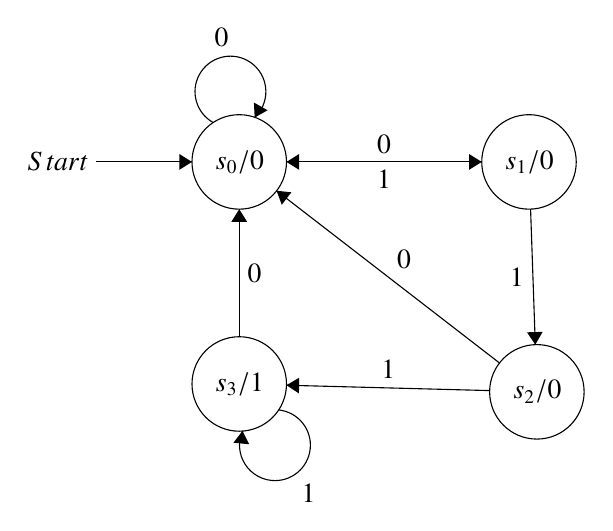
\begin{tikzpicture}[scale=0.2]
			\tikzstyle{every node}+=[inner sep=0pt]
			\draw [black] (15.5,-23.7) circle (3);
			\draw (15.5,-23.7) node {$s_0/0$};
			\draw [black] (33.9,-23.7) circle (3);
			\draw (33.9,-23.7) node {$s_1/0$};
			\draw [black] (34.4,-38.3) circle (3);
			\draw (34.4,-38.3) node {$s_2/0$};
			\draw [black] (15.5,-37.8) circle (3);
			\draw (15.5,-37.8) node {$s_3/1$};
			\draw [black] (6.4,-23.7) -- (12.5,-23.7);
			\draw (5.9,-23.7) node [left] {$Start$};
			\fill [black] (12.5,-23.7) -- (11.7,-23.2) -- (11.7,-24.2);
			\draw [black] (34,-26.7) -- (34.3,-35.3);
			\fill [black] (34.3,-35.3) -- (34.77,-34.49) -- (33.77,-34.52);
			\draw (33.6,-31.01) node [left] {$1$};
			\draw [black] (31.4,-38.22) -- (18.5,-37.88);
			\fill [black] (18.5,-37.88) -- (19.29,-38.4) -- (19.31,-37.4);
			\draw (24.96,-37.52) node [above] {$1$};
			\draw [black] (15.5,-34.8) -- (15.5,-26.7);
			\fill [black] (15.5,-26.7) -- (15,-27.5) -- (16,-27.5);
			\draw (16,-30.75) node [right] {$0$};
			\draw [black] (17.993,-39.448) arc (84.25644:-203.74356:2.25);
			\draw (19.9,-44.13) node [below] {$1$};
			\fill [black] (15.71,-40.78) -- (15.13,-41.53) -- (16.13,-41.63);
			\draw [black] (13.855,-21.205) arc (241.12502:-46.87498:2.25);
			\draw (14.38,-16.41) node [above] {$0$};
			\fill [black] (16.48,-20.88) -- (17.3,-20.42) -- (16.43,-19.93);
			\draw [black] (32.03,-36.47) -- (17.87,-25.53);
			\fill [black] (17.87,-25.53) -- (18.2,-26.42) -- (18.81,-25.63);
			\draw (25.96,-30.5) node [above] {$0$};
			\draw [black] (30.9,-23.7) -- (18.5,-23.7);
			\fill [black] (18.5,-23.7) -- (19.3,-24.2) -- (19.3,-23.2);
			\draw (24.7,-23.2) node [above] {$0$};
			\draw [black] (18.5,-23.7) -- (30.9,-23.7);
			\fill [black] (30.9,-23.7) -- (30.1,-23.2) -- (30.1,-24.2);
			\draw (24.7,-24.2) node [below] {$1$};
		\end{tikzpicture}
	\end{center}
\caption{FSM for Bitstream}
\label{fig:bitstream}
\end{figure}
Transition Table can be seen in Table. \ref{tab:bitstream}\\
\begin{table}[h!]
	
\begin{center}
	

\begin{tabular}{ |c|c|c|c|c|c| }
	\hline
	\multicolumn{2}{|c|}{Present State} &\multicolumn{1}{|c|}{Input} & \multicolumn{2}{|c|}{Next State} & \multicolumn{1}{|c|}{Output}  \\
	\hline
	A & B & x & $A^{\prime}$ & $B^{\prime}$ & y \\
	\hline
	0 & 0 & 0 & 0 & 0 & 0 \\
	\hline
	0 & 0 & 1 & 0 & 1 & 0 \\
	\hline
	0 & 1 & 0 & 0 & 0 & 0 \\
	\hline
	0 & 1 & 1 & 1 & 0 & 0 \\
	\hline
	1 & 0 & 0 & 0 & 0 & 0 \\
	\hline
	1 & 0 & 1 & 1 & 1 & 0 \\
	\hline
	1 & 1 & 0 & 0 & 0 & 1 \\
	\hline
	1 & 1 & 1 & 1 & 1 & 1 \\
	\hline
\end{tabular}
\end{center}
\caption{Transition Table for Bitstream}
\label{tab:bitstream}
\end{table}
from Fig. \ref{fig:kmap_da}
\begin{equation}
	D_a = Ax+Bx
\end{equation}
from Fig. \ref{fig:kmap_db}
\begin{equation}
	D_b = Ax+B^{\prime}x
\end{equation}
from Fig.  \ref{fig:kmap_y}
\begin{equation}
	y = AB 
\end{equation}
\begin{figure}[!h]
	\resizebox {\columnwidth} {!} {
		\begin{karnaugh-map}[4][2][1][][]
   \maxterms{0,1,2,4,6}
    \minterms{3,5,7}
    \implicant{3}{7}
    \implicant{5}{7}
    %\implicantedge{12}{8}{14}{10}
	%\indeterminants{10,11,12,13,14,15}        
    \draw[color=black, ultra thin] (0, 2) --
    node [pos=0.7, above right, anchor=south west] {$Bx$} % Y label
    node [pos=0.7, below left, anchor=north east] {$A$} % X label
    ++(135:1);
        
    \end{karnaugh-map}

	}
	\caption{K-map for $D_a$.}
	\label{fig:kmap_da}
\end{figure}
\begin{figure}[!h]
	\resizebox {\columnwidth} {!} {
		\begin{karnaugh-map}[4][2][1][][]
   \maxterms{0,2,3,4,6}
    \minterms{1,5,7}
    \implicant{1}{5}
    \implicant{5}{7}
    %\implicantedge{12}{8}{14}{10}
	%\indeterminants{10,11,12,13,14,15}        
    \draw[color=black, ultra thin] (0, 2) --
    node [pos=0.7, above right, anchor=south west] {$Bx$} % Y label
    node [pos=0.7, below left, anchor=north east] {$A$} % X label
    ++(135:1);
        
    \end{karnaugh-map}

	}
	\caption{K-map for $D_b$.}
	\label{fig:kmap_db}
\end{figure}
\begin{figure}[!h]
	\resizebox {\columnwidth} {!} {
		\begin{karnaugh-map}[4][2][1][][]
   \maxterms{0,1,2,3,4,5}
    \minterms{6,7}
    \implicant{7}{6}
   % \implicant{5}{7}
    %\implicantedge{12}{8}{14}{10}
	%\indeterminants{10,11,12,13,14,15}        
    \draw[color=black, ultra thin] (0, 2) --
    node [pos=0.7, above right, anchor=south west] {$Bx$} % Y label
    node [pos=0.7, below left, anchor=north east] {$A$} % X label
    ++(135:1);
        
    \end{karnaugh-map}

	}
	\caption{K-map for $y$.}
	\label{fig:kmap_y}
\end{figure}
\end{enumerate}



	
	
%\begin{figure}[!h]
	
%	\centering
%	\resizebox {\columnwidth} {!} {
%		\usepackage{pgf}
\usepackage{tikz}
%\usetikzlibrary{arrows,automata}
\usepackage[latin1]{inputenc}
%\usepackage{tikz}
\usetikzlibrary{arrows,automata, positioning, calc}
%\usetikzlibrary{arrows,automata, calc}
%\usetikzlibrary{arrows,automata}
\begin{tikzpicture}[->,auto] 
\node[state, initial] (1) {$s_0$};
\node[state, right of=1] (2) {$s_1$};
\node[state, right of=2] (3) {$s_2$};
\node[state, right of=3] (4) {$s_3$};
\node[state, right of=4] (5) {$s_4$};
\node[state, below of=5] (6) {$s_5$};
\node[state, left of=6] (7) {$s_6$};
\node[state, left of=7] (8) {$s_7$};
\node[state, left of=8] (9) {$s_8$};
\node[state, left of=9] (10) {$s_9$};


    
    % State relations 
  \path (1) edge node{} (10) 
  \path (10) edge node{} (9)
  \path (9) edge node{} (8)
  \path (8) edge node{} (7)
  \path (7) edge node{} (6)
 \path (6) edge node{} (5)
  \path (5) edge node{} (4)
 \path (4) edge node{} (3)
 \path (3) edge node{} (2)
  \path (2) edge node{} (1)
    ;
\end{tikzpicture}

%	}
%	\caption{FSM for the decade counter.}
%	\label{fig:fsm_down}
%\end{figure}
\bibliography{IEEEabrv,gvv_kmap_fsm}
\end{document}


